% !TEX program = xelatex
%%%%%%%%%%%%%%%%%%%%%%%%

\documentclass[11pt,aspectratio=169]{beamer} % 11pt is default
\usetheme{metropolis} % [progressbar=frametitle]
\setbeamercolor{background canvas}{bg=white}
\setbeamertemplate{caption}{\insertcaption} 
\setbeamersize{text margin left=2em,text margin right=2em}
\setbeamertemplate{frame footer}{\vspace{-5pt}}

\usepackage[round]{natbib}
\usepackage{amsmath}
\usepackage{mathtools}
\usepackage[group-minimum-digits=4,group-separator={,}]{siunitx}
\usepackage{graphicx}
\usepackage{wrapfig}
\usepackage{multimedia}

\usepackage{tikz}
\usetikzlibrary{backgrounds}
\usetikzlibrary{arrows,shapes}
\usetikzlibrary{tikzmark}
\usetikzlibrary{calc}
\usepackage[dvipsnames]{xcolor}

\usepackage[skins,theorems]{tcolorbox}
\usepackage{pdfpages}
\usepackage{colortbl}
\usepackage{changepage}
\usepackage{booktabs}
\usepackage{makecell}
\usepackage{setspace}
\usepackage{algorithm}
\usepackage[noend]{algpseudocode}
\usepackage{subcaption}
\usepackage[framemethod=TikZ]{mdframed}
\usepackage{xspace}

\usepackage{annotate-equations}

% Shortcut for beamer frames
\newcommand{\bframe}[2][c]{\begin{frame}[#1]{#2}}
\newcommand{\eframe}{\end{frame}} % \eframe causes problems for some reason

% Shortcut for bold text
\newcommand{\fat}[1]{\textbf{#1}}

% Boxing items on slide
\newcommand{\Cboxed}[2]{\colorlet{currentcolor}{.}{\color{#1}\fbox{\color{currentcolor}#2}}} %create coloured box around equation

% checkmark and xmark
\usepackage{pifont}
\newcommand{\cmark}{\ding{51}}%
\newcommand{\xmark}{\ding{55}}%

% Highlighting text in orange
\newcommand{\e}[1]{\alert{#1}}

% Underline
\newcommand{\uline}[1]{\underline{#1}}

% Include figure
\newcommand{\imgw}[2]{\includegraphics[width=#2\textwidth]{#1}} % \imgw{file}{height-scale}
\newcommand{\imgh}[2]{\includegraphics[height=#2\textheight]{#1}} % \imgh{file}{width-scale}

% Shortcut for latex commands
\newcommand{\blist}{\vspace{-3pt}\begin{list}{\raisebox{1pt}{\small$\bullet$}}{\leftmargin=13pt\itemsep=4pt}}
\newcommand{\blisttab}{\vspace{5pt}\blist}
\newcommand{\elisttab}{\end{list}}
\newcommand{\listtab}{\\[3pt] $\Rightarrow$ }
\newcommand{\elist}{\end{list}\vspace{5pt}}
\newcommand{\bblock}[1]{\metroset{block=fill}\begin{block}{#1}}
\newcommand{\eblock}{\end{block}}
\newcommand{\bmath}[1][0]{\begin{equation*}\hspace{#1em}}
\newcommand{\emath}{\end{equation*}}
\newcommand{\bcol}{\begin{columns}}
\newcommand{\col}[1]{\column{#1\textwidth}}
\newcommand{\tcol}[1]{\column[T]{#1\textwidth}}
\newcommand{\ecol}{\end{columns}}
\newcommand{\place}[4]{\begin{textblock}{#3}(#1,#2) #4 \end{textblock}} % \place{x}{y}{width}{text}
\newcommand{\placeframed}[4]{\place{#1}{#2}{#3}{\fbox{\parbox{#3em}{#4}}}}
\newcommand{\placeimg}[4]{\place{#1}{#2}{#3}{\imgw{#4}{1}}} % \placeimg{x}{y}{width}{file}
\newcommand{\videolink}[2]{\movie[externalviewer]{{\bf Video:} #1}{videos/#2}} % \videolink{title}{file}
\newcommand{\btab}[1]{\begin{tabular}{#1}}
\newcommand{\etab}{\end{tabular}}
\newcommand{\balgo}[2][1.3]{{#2:} \\[5pt] \begin{algorithmic}[1] \linespread{#1}\selectfont}
\newcommand{\ealgo}{\end{algorithmic}}
\renewcommand{\algorithmicloop}{\textbf{repeat:}}
\newcommand{\cred}{\cellcolor{red!25}}
\newcommand{\cgreen}{\cellcolor{green!25}}

% Shortcut for commonly used math symbols
\newcommand{\condpr}[2]{\text{Pr}\hspace{-1pt}\left\{ #1 \ \mid \ #2 \right\}}
\newcommand{\exarg}[2]{\mathbb{E}_{#1}\hspace{-2pt}\left[ #2 \right]}
\newcommand{\exnoarg}[1]{\mathbb{E}_{#1}}
\NewDocumentCommand\ex{ m g }{
	\IfNoValueTF{#2}{\exnoarg{#1}}{\exarg{#1}{#2}}
}
\newcommand{\der}[2]{\frac{\partial #1}{\partial #2}}
\newcommand{\stats}{\mathcal{S}}
\newcommand{\acts}{\mathcal{A}}
\newcommand{\rews}{\mathcal{R}}
\newcommand{\eps}{\mathcal{E}}
\newcommand{\ver}{\,\vert\,}
\newcommand{\vhat}{\hat{v}}
\newcommand{\qhat}{\hat{q}}
% \newcommand{\para}{\textbf{w}}
\newcommand{\feats}{\textbf{x}}
\newcommand{\elig}{\textbf{z}}
\newcommand{\gradient}{\nabla}
\newcommand{\outline}{Lecture Outline}
\newcommand{\reading}{Reading}
\newcommand{\h}[1]{\emph{#1}}

\emph
% \newcommand{\lindex}[1]{%
% 	\lowercase{\def\temp{#1}%
% 	\expandafter\index\expandafter{\temp}%
% }

\newcommand{\indx}[1]{\index{#1}}
\newcommand{\hind}[1]{\h{#1}\lindex{#1}}

% Set of real numbers
\newcommand{\R}{\mathbb{R}}
% Proportional to
% Transpose of a vector x
\newcommand{\vectranspose}[1]{#1^\top}
% Transpose of a matrix X
\newcommand{\mattranspose}[1]{#1^\top}
% Probability
\newcommand{\pr}{\text{Pr}}
% Conditional probability of x given y
\newcommand{\cpr}[2]{\pr( #1 \mid #2 )}
% x sampled according to probability distribution p
\newcommand{\sampled}[2]{#1 \sim #2}
% Assign value y to variable x
\newcommand{\assign}[2]{#1 \gets #2}
% Training data set
\newcommand{\data}{\mathcal{D}}
% Concatenation of inputs a, b, c, ...
\newcommand{\con}[1]{\langle #1 \rangle}
% array with bracket
\newcommand{\bra}[2]{\left[ \begin{array}{#1} #2 \end{array} \right]}
% Indicator function: returns 1 if x is true, otherwise returns 0
\newcommand{\ind}[1]{[#1]_1}

% common way of referring to places
\newcommand{\seehere}[1]{(\cref{#1})}

% shortcut text commands
\newcommand{\rl}{RL\xspace}
\newcommand{\marl}{MARL\xspace}
\newcommand{\ctde}{CTDE\xspace}
\newcommand{\sa}{single-agent\xspace}
\newcommand{\ma}{multi-agent\xspace}
\newcommand{\Ma}{Multi-agent\xspace}
\newcommand{\mas}{multi-agent system\xspace}
\newcommand{\stat}{stationarity\xspace}
\newcommand{\nonstat}{non-stationarity\xspace}
\newcommand{\pg}{policy gradient\xspace}
\newcommand{\vb}{value-based\xspace}
\newcommand{\pbt}{population-based training\xspace}
\newcommand{\psro}{policy space response oracles\xspace}
\newcommand{\Psro}{Policy space response oracles\xspace}
\newcommand{\sct}{\emph{StarCraft~II}\xspace}
\newcommand{\as}{AlphaStar\xspace}
\newcommand{\az}{AlphaZero\xspace}
\newcommand{\lbf}{level-based foraging\xspace}
\newcommand{\Lbf}{Level-based foraging\xspace}
\newcommand{\nfg}{normal-form game\xspace}
\newcommand{\nfgs}{normal-form games\xspace}
\newcommand{\Nfg}{Normal-form game\xspace}
\newcommand{\Nfgs}{Normal-form games\xspace}
\newcommand{\rps}{Rock-Paper-Scissors\xspace}
\newcommand{\pd}{Prisoner's Dilemma\xspace}
\newcommand{\survey}[4]{\noindent #1 (#4). ``#2.'' In: {\it #3}. \\}
\newcommand{\nashprob}{\textsc{Nash}\xspace}
\newcommand{\eol}{\textsc{End-of-Line}\xspace}
\newcommand{\ul}[1]{\underline{#1}}
\newcommand\norm[1]{\lVert#1\rVert}
\newcommand{\qlearn}{Q-learning\xspace}
\newcommand{\sarsa}{Sarsa\xspace}
\newcommand{\bayes}{Bayesian\xspace}
\newcommand{\bellman}{Bellman\xspace}
\newcommand{\markov}{Markov\xspace}
\newcommand{\pareto}{Pareto\xspace}
\newcommand{\boltzmann}{Boltzmann\xspace}
\newcommand{\mc}{Monte Carlo\xspace}
\newcommand{\nash}{Nash\xspace}
\newcommand{\ppad}{PPAD}
\newcommand{\dqn}{deep Q-networks\xspace}
\newcommand{\reinforce}{REINFORCE\xspace}
\newcommand{\qmix}{QMIX\xspace}
\newcommand{\qtran}{QTRAN\xspace}
\newcommand{\adam}{Adam\xspace}
\newcommand{\nret}{{$N$}-step returns\xspace}

% COMMANDS FOR COMMON NOTATION

% agent set
% state space
\newcommand{\St}{S}
\newcommand{\Stterm}{\bar{\St}}
% state
\newcommand{\st}{s}
\newcommand{\sth}{\hat{\st}}
% observation space
\newcommand{\Ob}{O}

% observation
\newcommand{\ob}{o}

% joint observation
\newcommand{\job}{o}
% action space
\newcommand{\Ac}{A}

% action
\newcommand{\ac}{a}
\newcommand{\ach}{\hat{\ac}}

% joint action
\newcommand{\jac}{a}
% reward
\newcommand{\rew}{r}
\newcommand{\rewh}{\hat{\rew}}
% centralised information
\newcommand{\ci}{z}

% initial state distribution

\newcommand{\instdist}{\mu}
% % state transition function

\newcommand{\Stf}{\mathcal{T}}
% % simulation/sampling model
\newcommand{\Stfsim}{\widehat{\Stf}}

% observation function
\newcommand{\Obf}{\mathcal{O}}

% reward function
\newcommand{\Rew}{\mathcal{R}}

% POLICIES, RETURNS, VALUES

% policy space
\newcommand{\Pol}{\Pi}

% policy
\newcommand{\pol}{\pi}
\newcommand{\poltil}{\tilde{\pol}}

% set of histories
\newcommand{\His}{H}
\newcommand{\Fhis}{\hat{\His}}
% history
\newcommand{\his}{h}

% full history
\newcommand{\fhis}{\hat{\his}}

% observation history extracted from full history
\newcommand{\obsext}{\sigma}

% discount factor
\newcommand{\dsc}{\gamma}

% return
\newcommand{\ret}{u}

% expected return for joint policy
\newcommand{\exret}{U}

% Agents
\newcommand{\Ag}{I}

% RL / MARL

% learning algorithm

\newcommand{\alg}{\mathbb{L}}

% empirical distribution/ average policy
\newcommand{\empdis}{\bar{\pol}}
\newcommand{\avgpol}{\bar{\pol}}
\newcommand{\agmod}{\hat{\pol}}
\newcommand{\Agmod}{\hat{\Pol}}
\newcommand{\agmodj}{agent model for agent $j$}

% best response
\newcommand{\br}{\textnormal{BR}}

% game value
\newcommand{\gval}{Value}

% value under agent model
\newcommand{\amval}{AV}

% regret
\newcommand{\regret}{Regret}
\newcommand{\avgreg}{\bar{R}}
% TD target
\newcommand{\target}{\mathcal{X}}
% step size (for gradient-based MARL in Chapter 5)
\newcommand{\step}{\kappa}


% DEEP LEARNING

% parameters
\newcommand{\para}{\theta}

% loss
\newcommand{\loss}{\mathcal{L}}
% batch
\newcommand{\batch}{\mathcal{B}}
\newcommand{\batchsize}{B}

% etnropy
\newcommand{\entropy}{\mathcal{H}}

% Create algorithm environment
\newcommand{\balg}[2]{
  \begin{algorithm}[H]
    \caption{#1}
    \label{alg:#2}
    \setstretch{1.1}
    \begin{algorithmic}[1]}

\newcommand{\ealg}{
    \end{algorithmic}
  \end{algorithm}}

% Argmin/ Argmax operators

\DeclareMathOperator*{\argmin}{arg\,min} 
\DeclareMathOperator*{\argmax}{arg\,max}

\makeatletter
\newenvironment{myitemize}{%
   \setlength{\topsep}{0pt}
   \setlength{\partopsep}{0pt}
   \renewcommand*{\@listi}{\leftmargin\leftmargini \parsep\z@ \topsep\z@ \itemsep\z@}
   \let\@listI\@listi
   \itemize
}{\enditemize}
\makeatother  

% define widebar for target parameters
\makeatletter
\newcommand*\rel@kern[1]{\kern#1\dimexpr\macc@kerna}
\newcommand*\widebar[1]{%
	\begingroup
	\def\mathaccent##1##2{%
		\rel@kern{0.8}%
		\overline{\rel@kern{-0.8}\macc@nucleus\rel@kern{0.2}}%
		\rel@kern{-0.2}%
	}%
	\macc@depth\@ne
	\let\math@bgroup\@empty \let\math@egroup\macc@set@skewchar
	\mathsurround\z@ \frozen@everymath{\mathgroup\macc@group\relax}%
	\macc@set@skewchar\relax
	\let\mathaccentV\macc@nested@a
	\macc@nested@a\relax111{#1}%
	\endgroup
}
\makeatother


% MATRIX GAMES

\newcolumntype{?}{!{\vrule width 1pt}}
\newcommand{\bhline}{\Xhline{1pt}}
\newcommand{\gametwo}[3]{
	\begin{tabular}{c?c|c}
		 & #1 \\
		\bhline
		#2    \\
		\hline
		#3    \\
	\end{tabular}
}
\newcommand{\gamethree}[4]{
	\begin{tabular}{c?c|c|c}
		 & #1 \\
		\bhline
		#2    \\
		\hline
		#3    \\
		\hline
		#4    \\
	\end{tabular}
}

\newcommand{\gamepd}{
    % \gametwo{C & D}{C & -1,-1 & -5,0}{D & 0,-5 & -3,-3}
	\begin{tabular}{c|c|c}
	& C & D \\
	\hline
	C & -1,-1 & -5,0 \\
	\hline
	D & 0,-5 & -3,-3
	\end{tabular}
}

\newcommand{\gamerps}{
    % \gamethree{R & P & S}{R & 0,0 & -1,1 & 1,-1}{P & 1,-1 & 0,0 & -1,1}{S & -1,1 & 1,-1 & 0,0}
	\begin{tabular}{c|c|c|c}
	& R & P & S \\
	\hline
	R & 0,0 & -1,1 & 1,-1 \\
	\hline
	P & 1,-1 & 0,0 & -1,1 \\
	\hline
	S & -1,1 & 1,-1 & 0,0
	\end{tabular}
}

\newcommand{\gamecoord}{
    % \gametwo{A & B}{A & 10 & 0}{B & 0 & 10}
	\begin{tabular}{c|c|c}
		& A & B \\
		\hline
		A & 10 & 0 \\
		\hline
		B & 0 & 10 \\
	\end{tabular}
}

\newcommand{\gamechicken}{
    % \gametwo{S & L}{S & 0,0 & 7,2}{L & 2,7 & 6,6}
	\begin{tabular}{c|c|c}
		& S & L \\
		\hline
		S & 0,0 & 7,2 \\
		\hline
		L & 2,7 & 6,6
	\end{tabular}
}

\newcommand{\gamestaghunt}{
    % \gametwo{S & H}{S & 4,4 & 0,3}{H & 3,0 & 2,2}
	\begin{tabular}{c|c|c}
		& S & H \\
		\hline
		S & 4,4 & 0,3 \\
		\hline
		H & 3,0 & 2,2
	\end{tabular}
}

\newcommand{\gamebattle}{
    \begin{tabular}{c|c|c}
    & A & B \\
    \hline
    A & 10,7 & 2,2 \\
    \hline
    B & 0,0 & 7,10
    \end{tabular}
}

\newcommand{\gameepsne}{
    % \gametwo{C & D}{A & 100,100 & 0,0}{B & 1,2 & 1,1}
	\begin{tabular}{c|c|c}
		& C & D \\
		\hline
		A & 100,100 & 0,0 \\
		\hline
		B & 1,2 & 1,1
	\end{tabular}
}

% Define colorboxes
\tcbset{
  % Defaults
  my box/main style/.style={},
  my box/title style/.style={},
  % Use the 'append' variants if you want to add to the defaults instead of
  % overriding them.
  my box/main/.style={/tcb/my box/main style/.style={#1}},
  my box/title/.style={/tcb/my box/title style/.style={#1}},
  my box/append main/.style={/tcb/my box/main style/.append style={#1}},
  my box/append title/.style={/tcb/my box/title style/.append style={#1}},
  %
  my box/.style={
    my box/.cd, #1,
    /tcb/.cd,
    enhanced,
    my box/main style,
    attach boxed title to top left={xshift=0.2cm, yshift=-0.2cm},
    top=10pt,
    boxed title style={
      outer arc=0pt,
      arc=0pt,
      top=3pt,
      bottom=3pt,
      my box/title style,
    },
  },
}

% define 'solutionbox' environment with coloured box
\newtcolorbox{solutionbox}[1][]{
  my box={
    main={colframe=green!40!gray!90, colback=green!20!gray!5},
    title={colback=green!40!gray!90},
  },
  title=Solution,
  #1,
}

\newtcolorbox{problembox}[1][]{
  my box={
    main={colframe=red!40!gray!90, colback=red!20!gray!5},
    title={colback=red!40!gray!90},
  },
  title=Problem,
  #1,
}

\newtcolorbox{notebox}[1][]{
  my box={
    main={colframe=orange!40!gray!80, colback=orange!20!gray!5},
    title={colback=orange!40!gray!80},
  },
  title=Note,
  #1,
}

\newtcolorbox{intuitionbox}[1][]{
  my box={
    main={colframe=blue!60!gray!80, colback=blue!20!gray!5},
    title={colback=blue!60!gray!80},
  },
  title=Intuition,
  #1,
}

\newtcolorbox{reminderbox}[1][]{
  my box={
    main={colframe=black!40!gray, colback=gray!10!white},
    title={colback=black!40!gray},
  },
  title=Reminder,
  #1,
}

\newtcolorbox{custombox}[2][]{
  my box={
    main={colframe=black!40!gray, colback=gray!10!white},
    title={colback=black!40!gray},
  },
  title={#2},
  #1,
}

% no title boxes
\newtcolorbox{greenbox}[1][]{
  my box={
    main={colframe=green!40!gray!90, colback=green!20!gray!5},
  },
  #1,
}
\newtcolorbox{redbox}[1][]{
  my box={
    main={colframe=red!40!gray!90, colback=red!20!gray!5},
  },
  #1,
}
\newtcolorbox{orangebox}[1][]{
  my box={
    main={colframe=orange!40!gray!80, colback=orange!20!gray!5},
  },
  #1,
}
\newtcolorbox{bluebox}[1][]{
  my box={
    main={colframe=blue!60!gray!80, colback=blue!20!gray!5},
  },
  #1,
}
\newtcolorbox{blackbox}[1][]{
  my box={
    main={colframe=black!55!black, colback=gray!5!white},
  },
  #1,
}


% Define intro slide command
\newcommand{\introslide}{
    \begin{frame}{MARL Book}
        \begin{columns}
            \begin{column}{0.5\textwidth}
            \begin{figure}
              \centering
              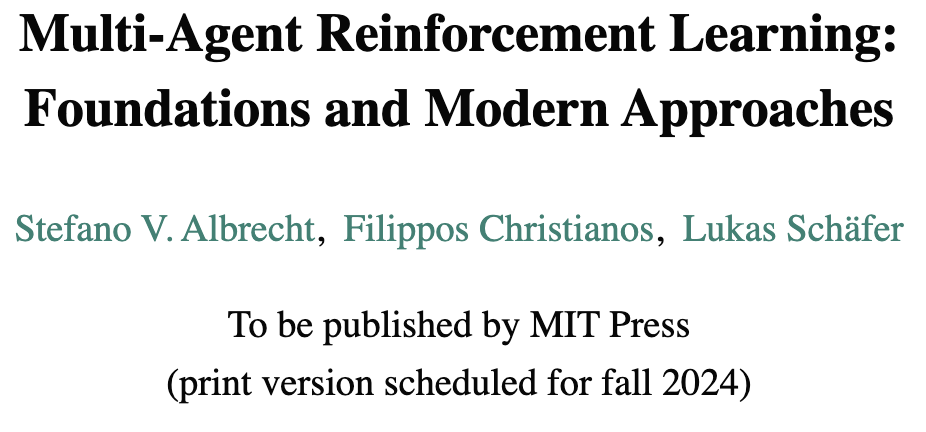
\includegraphics[width=\textwidth,height=.8\textheight,keepaspectratio]{images/1_MARL_book.png}
            
              \label{fig:enter-label}
            \end{figure}
          \end{column}
        
        \hspace{20pt}
            
          % Column for the text
            \begin{column}{0.45\textwidth}
	        \small

                This lecture is based on \textit{Multi-Agent Reinforcement Learning: Foundations and Modern Approaches} by Stefano V. Albrecht, Filippos Christianos and Lukas Sch\"afer
                
                \vspace{20pt}
                
                The book can be downloaded for free at \textcolor{blue}{\href{https://www.marl-book.com/}{www.marl-book.com}}.
            \end{column}
        
        \end{columns}
    \end{frame}
}

\newcommand{\leoslide}{
  \author{Stefano V. Albrecht, Filippos Christianos, Lukas Sch\"afer \\ Slides by: Leonard Hinckeldey}
}

\newcommand{\otherslide}{
  \author{Stefano V. Albrecht, Filippos Christianos, Lukas Sch\"afer}
}
	
\title{Multi-Agent Reinforcement Learning}
\date{}

\hypersetup{
  pdfsubject = {Multi-Agent Reinforcement Learning},
}

\leoslide

\subtitle{Multi-Agent Reinforcement Learning in Games: First Steps and Challenges}

\begin{document}
\maketitle

\introslide

\begin{frame}{\outline}

\blist
    \item Learning framework for MARL
    \item Independent learning
    \item Central learning
    \item Modes of learning
    \item Challenges of MARL
\elist
\end{frame}

\section{MARL Learning Framework}

\begin{frame}[t]{MARL Learning Process}

\begin{figure}
    \centering
    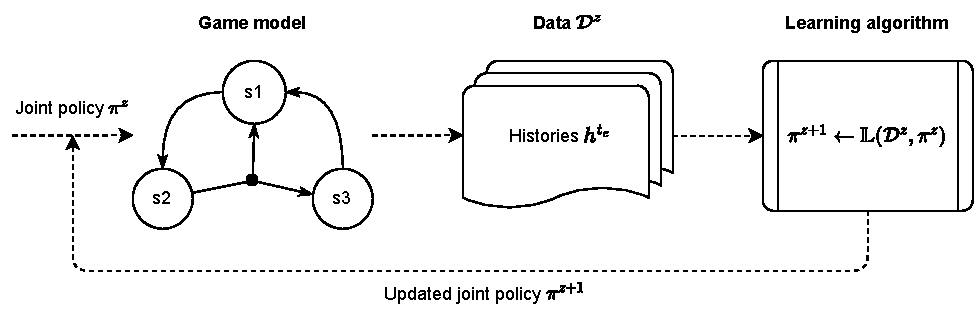
\includegraphics[width=0.8\textwidth, height = 0.8\textheight, keepaspectratio]{images/chapter_5/learning-process.pdf}
\end{figure}

\blist
    \item The game model defines the learning environment
    \item Interaction data from joint policy $\pol^z$ are collected as $\mathcal{D}^{z} = \{ h^{t_e} \mid e = 1, \ldots, z\}, z \geq 0$
    \item A learning algorithm updates the joint policy as $\pi^{z+1} = \mathbb{L}(\mathcal{D}^{z}, \pi^{z})$
    \item The learning goal is a chosen solution concept, e.g. Nash equilibrium
\elist
    
\end{frame}

% \begin{frame}{MARL Learning Process - Continued}

% There are several additional nuances to the MARL learning process.

% \blist
%     \item The chosen game model will determine what the learnt joint policy conditions on:
%     \vspace{-15pt}
%     \begin{itemize}
%         \item Normal-form games: simple probability distribution across actions
%         \item Repeated normal-form games: condition on action histories $h^t = (a^0, ..., a^{t–1})$
%         \item Stochastic games: condition on state-action histories $h^t = (s^0, a^0, s^1, a^1, ..., s^t)$
%         \item POSG: condition on independent observation histories $h^t_i = (o_i^0, ..., o^t_i)$
%     \end{itemize}
%     \item Policies can however be adjusted as required e.g. in a stochastic game only condition on the last state-action 
%     \item The learning algorithm $\mathbb{L}$ can consists of multiple learning algorithms e.g. $\mathbb{L}_i \forall i \in I$
%     \item Each $\mathbb{L}_i$ may use different parts of the data, or use independently collected data
% \elist

% \end{frame}

\begin{frame}[t]{Inputs of Policies Depend on Game Model}

% The chosen game model will determine what the learnt joint policy conditions on:

    \begin{minipage}[t]{0.39\linewidth}
        % First Column
        \centering
        \vspace{0.5cm}
        \visible<1->{
            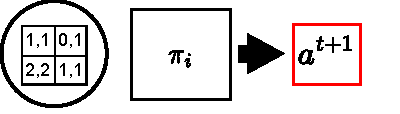
\includegraphics[width=0.8\linewidth, keepaspectratio]{images/chapter_4/nf_inputs-1.pdf}
            \textbf{Normal-form games}
        }
        \vspace{1.5cm}
        \visible<2->{
            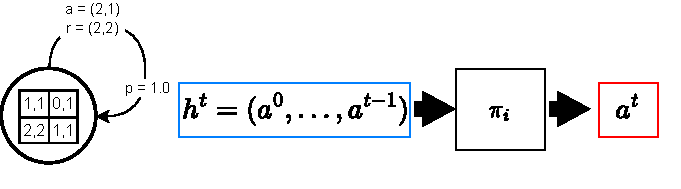
\includegraphics[width=\linewidth]{images/chapter_4/rnf_input-1.pdf} 
            \textbf{Repeated normal-form \\ games}
        }
    \end{minipage}
    \hfill
    \begin{minipage}[t]{0.59\linewidth}
        \centering
        \visible<3->{
            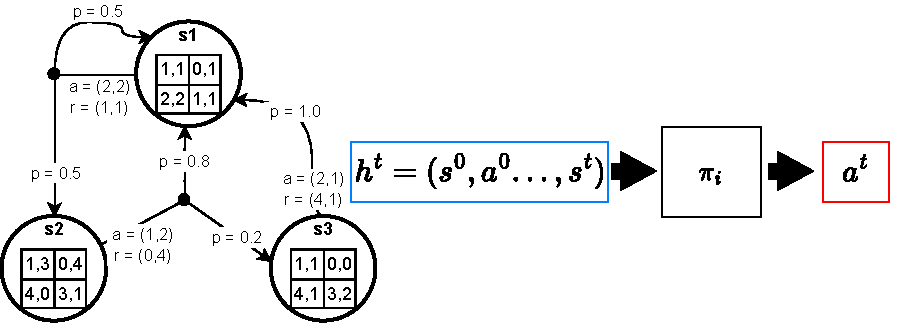
\includegraphics[width=0.75\linewidth]{images/chapter_4/sg_input-1.pdf}\\
            \textbf{Stochastic games}
        }
        \vspace{0.5cm}
        \visible<4->{
            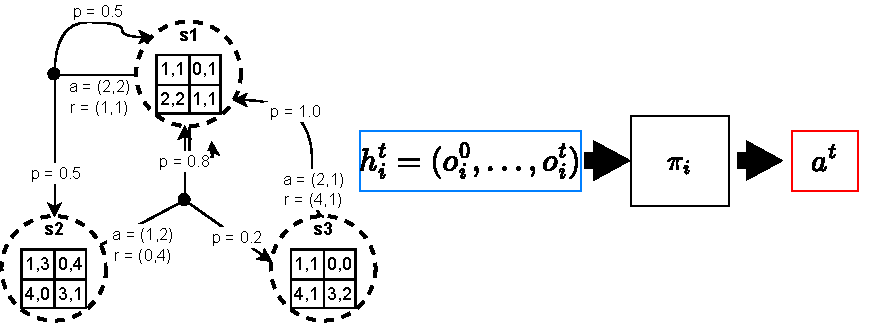
\includegraphics[width=0.75\linewidth]{images/chapter_4/posg_input-1.pdf}\\
            \textbf{Partially observable stochastic games}
        }
    \end{minipage}

\end{frame}

\begin{frame}{Convergence}

To evaluate the learning algorithm, we typically assess whether the learnt joint policy has \fat{converged} to an optimal joint policy:
\vspace{0pt}
\[
\lim_{z \to \infty}\pi^z = \pi^*
\]

\blist
    \item Optimal joint policies may differ depending on the solution concept
    \item There may be many valid solutions $\Rightarrow$ e.g. multiple Nash equilibria
    \item In practice, we cannot collect infinite data $z \to \infty$
    \listtab Learning typically stops after a predefined 'budget' (e.g. training steps)
    % \item Alternative theoretical evaluation criteria include:
    % \begin{itemize}
    %     \item Convergence of average return
    %     \item Convergence of empirical distribution of the learn policy to the optimal policy
    % \end{itemize}
\elist
    
\end{frame}


\begin{frame}[t]{Single-Agent RL Reductions}

The simplest way to apply RL algorithms in multi-agent settings is to reduce them to single-agent problems. 

\vspace{10pt}

\visible<2->{
\e{\bf Central learning:}
\blist
    \item Apply one single-agent RL algorithm to control all agents centrally 
    \listtab A central policy is learned over the joint action space
\elist}

\visible<3->{
\e{\bf Independent learning:}
\blist
    \item Apply single-agent RL algorithms to each agent independently
	\listtab Agents do not explicitly consider or represent each other
\elist}
    
\end{frame}

\section{Central Learning}

\begin{frame}{Central Learning}

\e{Central learning:} learn a single central policy $\pi_c$ which receives observations of all agents and selects an action for each agent (i.e. joint action $(\ac_1,...,\ac_n)$). 

\blist
    \item<1-> Requires transforming the joint reward $(r_1, \ldots, r_n)$ into a single scalar reward $r$
    \item<2-> This can be easy in some settings, e.g. in games with common rewards $r = r_i$, but difficult in zero-sum or general-sum games
    \item<3-> Mays not scale well with the number of agents, as the joint action space may grow exponentially with the number of agents
    \item<4-> May also not be suitable in environments that require agents to act independently based on local observations
\elist
\end{frame}

\begin{frame}{Central Q-Learning}


\balg{Central Q-learning}{cql}
\State Initialize: \( Q(s, a) = 0 \) for all \( s \in S \) and \( a \in A = A_1 \times \ldots \times A_n \)
\State Repeat for every episode:
\For{\( t = 0, 1, 2, \ldots \)}
    \State Observe current state \( s^t \)
    \State With probability \( \epsilon \): choose random joint action \( a^t \in A \)
    \State Otherwise: choose joint action \( a^t \in \arg\max_a Q(s^t, a) \)
    \State Apply joint action \( a^t \), observe rewards \( r_1^t, \ldots, r_n^t \) and next state \( s^{t+1} \)
    \State Transform \( r_1^t, \ldots, r_n^t \) into scalar reward \( r^t \)
    \State \( Q(s^t, a^t) \leftarrow Q(s^t, a^t) + \alpha [ r^t + \gamma \max_{a'} Q(s^{t+1}, a') - Q(s^t, a^t) ] \)
\EndFor
\ealg

\end{frame}

\section{Independent Learning}

\begin{frame}{Independent Learning}

\e{Independent learning:} each agent $i$ learns its policy $\pi_i$ using only its local history of observations.

\blist
    \item From the perspective of each agent $i$, the environment transition function looks like this:
\elist
\[
\mathcal{T}_i(s^{t+1} | s^t, a_i) \propto \sum_{a_{-i} \in A_{-i}} \mathcal{T}(s^{t+1} | s^t, \langle a_i, a_{-i} \rangle) \prod_{j \neq i} \pi_j(a_j | s^t)
\]
% \vspace{5pt}
\blist
    \item As each agent $j$'s policies are updated, the action probabilities $\pi_j$ change
    \listtab From agent $i$'s perspective, the transition function $\mathcal{T}_i$ appears non-stationary!
\elist
    
\end{frame}

\begin{frame}{Independent Q-learning}

\balg{Independent Q-learning (IQL) for stochastic games}{iql}
\State // \textit{Algorithm controls agent} \( i \)
\State Initialize: \( Q_i(s, a_i) = 0 \) for all \( s \in S \), \( a_i \in A_i \)
\State Repeat for every episode:
\For{\( t = 0, 1, 2, \ldots \)}
    \State Observe current state \( s^t \)
    \State With probability \( \epsilon \): choose random action \( a_i^t \in A_i \)
    \State Otherwise: choose action \( a_i^t \in \arg\max_{a_i} Q_i(s^t, a_i) \)
    \State (meanwhile, other agents \( j \neq i \) choose their actions \( a_j^t \))
    \State Observe own reward \( r_i^t \) and next state \( s^{t+1} \)
    \State \( Q_i(s^t, a_i^t) \leftarrow Q_i(s^t, a_i^t) + \alpha [ r_i^t + \gamma \max_{a'_i} Q_i(s^{t+1}, a'_i) - Q_i(s^t, a_i^t) ] \)
\EndFor
\ealg
\end{frame}

\begin{frame}{IQL and CQL in Level-Based Foraging}

\begin{columns}
    \begin{column}{0.5\textwidth}
    \begin{figure}
        \centering
        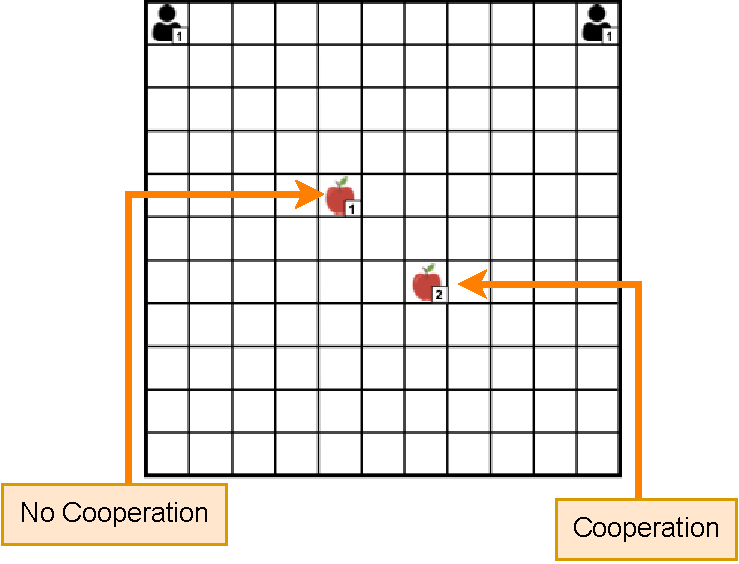
\includegraphics[width=\textwidth,height=.8\textheight,keepaspectratio]{images/environments/lbf/tabular_marl_lbf_annot.pdf}
        \label{fig:enter-label}
        
    \end{figure}
        
    \end{column}
    
    \begin{column}{0.5\textwidth}
    \vspace{10pt}
        \centering
        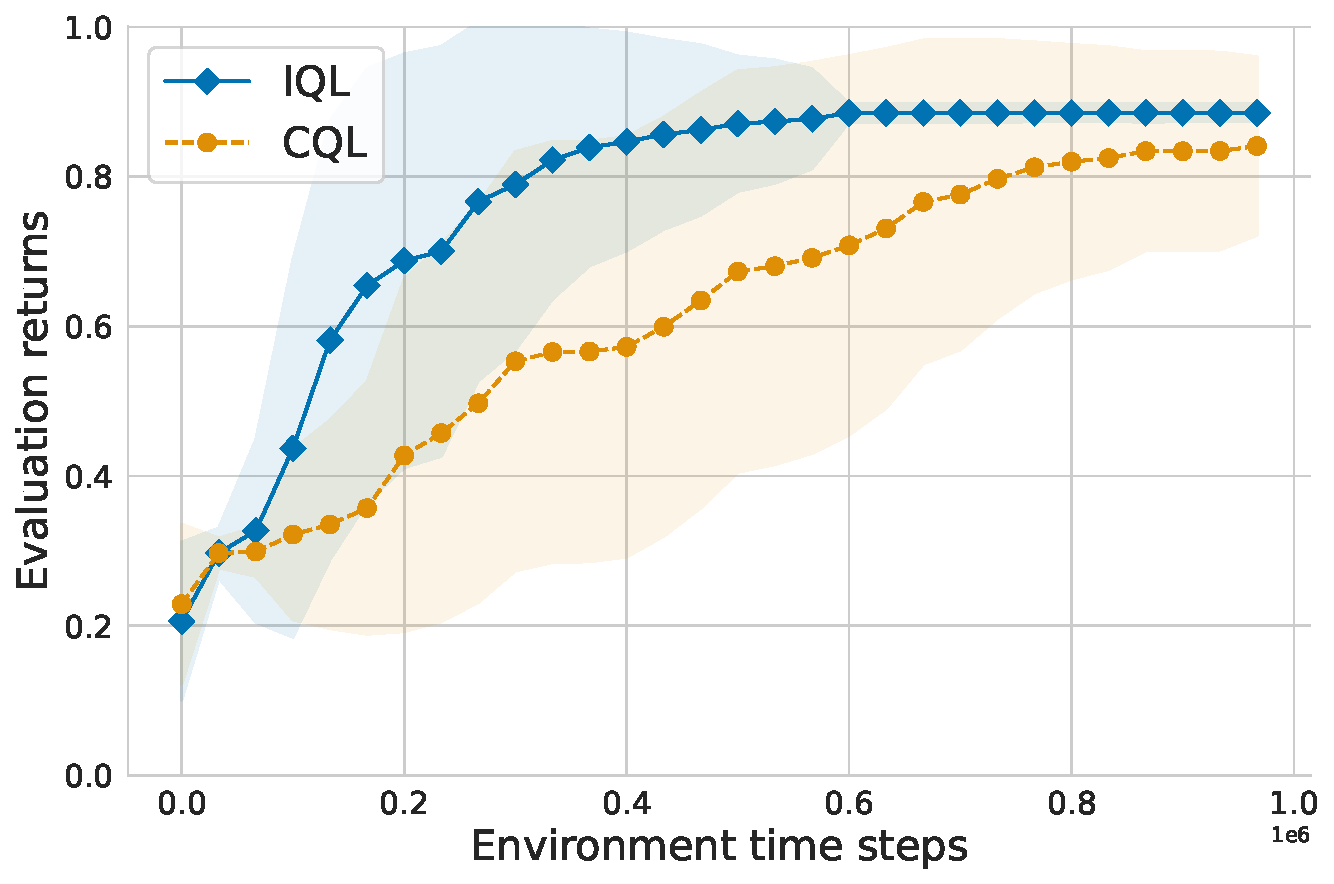
\includegraphics[width=\textwidth,height=.8\textheight,keepaspectratio]{images/chapter_5/tabular_marl_lbf_returns_iql_cql.pdf}
        \label{fig:enter-label}
        \blist
            \item IQL can learn more quickly, as CQL needs to explore $6^2 = 36$ actions in each state
        \elist
        
    \end{column}
\end{columns}
    
\end{frame}

\begin{frame}{Modes of Operation in MARL}

Modes of Operation in MARL: \fat{self-play} and \fat{mixed-play}

\vspace{10pt}

\fat{Self-play}:
\blist
    \item \fat{Algorithm self-play:} all agents use the same learning algorithm (and parameters)
    \item \fat{Policy self-play:} agent's policy is trained directly against itself
\elist

\vspace{5pt}

\fat{Mixed-play}
\blist
    \item Agents use different learning algorithms
    % \item Trading bots in markets that use RL are one example of a mixed-play scenario
    % \item Ad-hoc teamwork is another area of research that focuses on this setting where agents must collaborate with previously unknown agents
\elist
    
\end{frame}

\section{MARL Challenges}

\begin{frame}{MARL Challenges}

\small 

\bcol
	\tcol{0.47}
		\begin{custombox}{Singe-Agent RL Challenges}
		\blist
		    \item Unknown environment dynamics
		    \item Exploration-exploitation dilemma
		    \item Non-stationarity from bootstrapping
		    \item Temporal credit assignment
		\elist
		\end{custombox}
		
	\tcol{0.5}
		\visible<2->{
		\begin{custombox}{Multi-Agent RL Challenges}
		\blist
		    \item Non-stationarity from multiple learning agents
   		    \item Equilibrium selection
		    \item Multi-agent credit assignment
		    \item Scaling tom many agents
		\elist
		\end{custombox}
		}
\ecol    
\end{frame}

\begin{frame}{Non-Stationarity}

\underline{A stochastic process ${X^t}_{t \in \mathbb{N}^0}$ is stationary if:}

\begin{itemize}
    \item The probability distribution of $X^{t + \tau}$ does not depend on $\tau \in \mathbb{N}^0$, where t and $t + \tau$ are time indices
    \item This means that the dynamics of the process do not change over time
\end{itemize}

\pause

\underline{Consider: $X^t$ samples the state $s^t$ at each time step $t$:}

\begin{itemize}
    \item<2-> In a MDP, $X^t$ is completely defined by the state transition function $\mathcal{T}(s^t|s^{t-1}, a^{t-1})$ and the agent's policy $\pi$ which selects an action $a \sim \pi(.|s)$
    \item<3-> If $\pi$ does not change, then this process is stationary (i.e. independent of $t$) because $s^t$ depends only on $s^{t-1}$, $a^{t-1}$ and $a^{t-1}$ depends only on  $s^{t-1}$ via $\pi(.|s^{t-1})$
    \item<4-> However, in RL the policy does change over time through the learning $\pi^{z+1} = \mathbb{L}(\mathcal{D}^z, \pi^z)$,  which leads to \fat{non-stationarity} in $X^t$
\end{itemize}

\end{frame}

\begin{frame}[t]{Non-Stationarity in Multi-Agent Settings}

In MARL, non-stationarity is exacerbated by multiple agents changing their policies!

\vspace{15pt}

\bcol
	\col{0.45}
        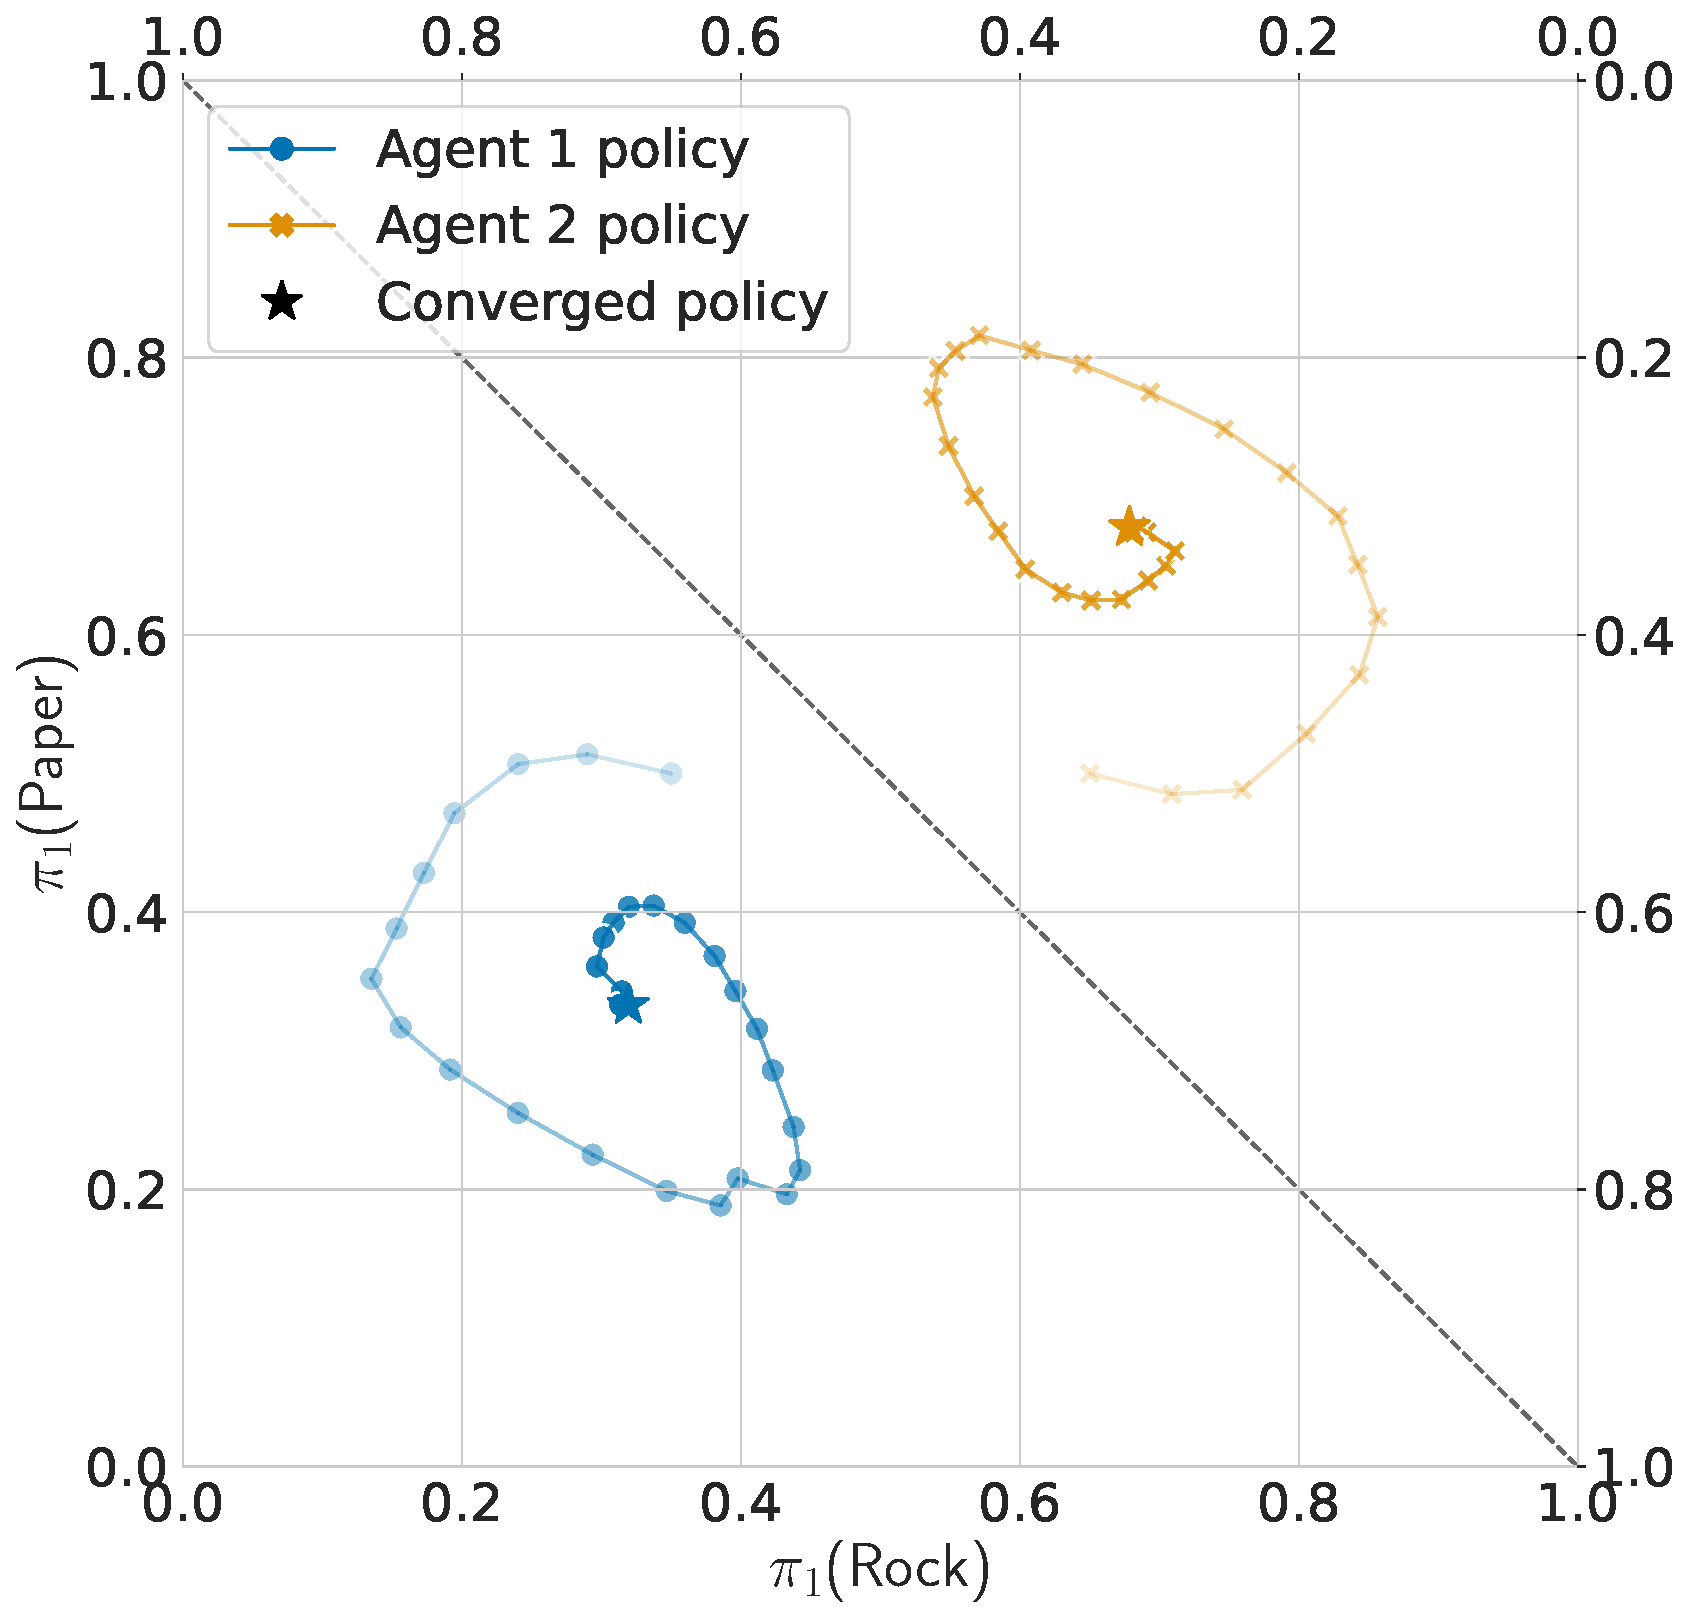
\includegraphics[width=0.95\textwidth]{images/chapter_5/wolfphc_rps_own.pdf}

	\col{0.45}
		\blist
		    \item $\pi^{z+1} = \mathbb{L}(\mathcal{D}^z, \pi^z)$ updates an {\it entire} joint policy $\pi^z = (\pi_1^z, ..., \pi_n^z)$
		    \item Environment is non-stationary from each agent's perspective
		    \item Can cause cyclic learning dynamics where agents co-adapt to each other's changing policies 
		    % \item Stochastic approximation conditions that ensure convergence in single-agent RL don't apply in MARL
		\elist

\ecol
\end{frame}

\begin{frame}{Equilibrium Selection}

\e{\bf Equilibrium selection:} a game may have multiple equilibria, which can yield different expected returns to the agents.
\vspace{5pt}

\bcol
    \col{0.5}
        \blist
            \item<1-> {\bf Example:} Stag Hunt matrix game
            \item<1-> Two hunters choose: cooperate to hunt stag (S) or go solo for hare (H)
            \item<2-> Nash equilibria: reward-dominant (S,S) maximizes reward, risk-dominant (H,H) minimizes risk
            \item<3-> (S,S) requires trust; (H,H) offers a safe, lower reward
        \elist

    \col{0.5}
        \centering
        \gamestaghunt
		\vspace{10pt}
		\visible<4->{
        \blist
            \item Indep. Q-learning may bias towards (H,H) due to initial action uncertainty
            \item Early random actions can reinforce (H,H) since deviating from H is penalized if the other agent chooses H
        \elist}

\ecol
    
\end{frame}

\begin{frame}{Multi-Agent Credit Assignment}

%Credit assignment in single-agent RL refers to determining which past action contributes to receiving rewards.
\e{\bf Multi-agent credit assignment:} which agent's actions contributed to receved rewards? \\[15pt]

\bcol
    \col{0.5}
            \centering
            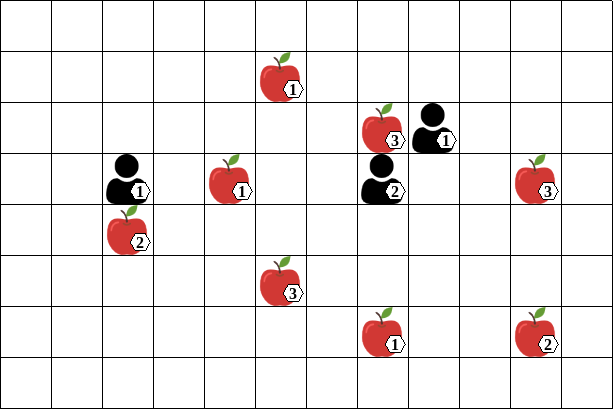
\includegraphics[width=0.85\textwidth]{images/environments/lbf/foraging_8x12_b.png}

    \col{0.5}
        \blist
            \item At time step $t$ all agents perform \textit{collect}, each receiving reward $+1$
            \item Whose actions led to the reward?
            \item The agent on the left did not contribute
            \item For a learning agent that only observes $s^t, a^t, r^t, s^{t+1}$, disentangling the action contributions is difficult
        \elist

\ecol
    
\end{frame}
\begin{frame}[t]{Joint Actions for Addressing Multi-Agent Credit Assignment}

\fat{Joint actions} can help disentangle agent contributions. Consider the RPS game:

\vspace{5pt}

\centering
\gamerps 

\vspace{5pt}

\begin{enumerate}
    \item<2-> Agents choose actions $(a_1, a_2) = (R, S)$ $\quad\Rightarrow$ agent $1$ receives reward $+1$
    \item<3-> Then agents choose $(a_1, a_2) = (R, P)$ $\quad\Rightarrow$ agent $1$ receives reward $-1$
    \item<4-> Action value $Q(a_1)$ does not model agent $2$, value for action $R$ appears to be 0
    \item<5-> \e{Joint action value model} $Q_1(a_1, a_2)$ can represent the effect of agent $2$: $Q_1(R, S)=+1$ and $Q_1(R, P)=-1$
\end{enumerate}

\end{frame}

\begin{frame}{Scaling to Many Agents}

    \begin{problembox}
	    \blist
	        \item \textbf{Joint action space} can grow \textbf{exponentially} with number of agents:
	        	$$|A| = |A_1| \cdot ... \cdot |A_n|$$
	        \item If agents have associated features in $s$ (e.g. agent position) then $|S|$ also increases exponentially
	        %\item In CL, this increases the decision problem, while in IL this increases issues of non-stationarity and multi-agent credit assignment
	        \listtab How to scale efficiently to many agents?
	    \elist
    \end{problembox}

\end{frame}

\begin{frame}{Scaling to Many Agents}
	    
	\bcol
	    \col{0.45}
	        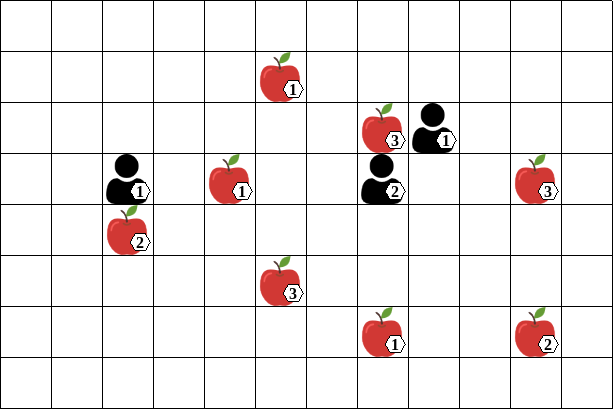
\includegraphics[width=0.9\textwidth]{images/environments/lbf/foraging_8x12_b.png}
	        
	    \col{0.45}
	        %\blist
	        	Changing number of agents from 3 to 5 increases the number of joint actions from 216 to 7776!
	        %\elist
	\ecol

\end{frame}

\begin{frame}{Summary}

\fat{We covered:}
    \blist
        \item MARL learning process
        \item Independent and central learning
        \item Modes of operation in MARL
        \item Challenges of MARL
    \elist

\fat{Next we'll cover:}

    \blist
        \item Foundational algorithms in MARL
    \elist
    
\end{frame}

\end{document}

